\documentclass[a4paper,11pt]{article}

\usepackage{amsmath}
\usepackage{amssymb}

% for proofs  environment
\usepackage{amsthm}

% for 3d plots
\usepackage{pgfplots}
\usepackage{pgfplotstable}
\usepgfplotslibrary{patchplots}

\usepackage[backend=bibtex]{biblatex}
\bibliography{reading7think}

% for probability trees
\usepackage{tikz}
\usetikzlibrary{trees}

% for Venn diagrams
\usetikzlibrary{shapes,backgrounds}
% for plots
\usepackage{ pgfplots}
% inserted on suggestion in warning during compilation
\pgfplotsset{compat=1.9}

%for strikethrough text
\usepackage{soul}

%for R source code listing
\usepackage{listings}

%for block quotes
\usepackage{csquotes}

% For not indenting the first line of paragraphs:
\setlength{\parindent}{0pt}
% define the title
\author{John Hancock}
\title{MIT Introduction to Statistics 18.05 Reading 7 Think Questions}
\begin{document}
% generates the title
\maketitle
% insert the table of contents
\tableofcontents
\section{References and License}
We are answering questions in the material from MIT OpenCourseWare
course 18.05, Introduction to Probability and Statistics.

In this document we are answering questions Orloff and Bloom ask in
\cite{reading7}.

Please see the references section for detailed citation information.

The material for the course is licensed under the terms at
\url{http://ocw.mit.edu/terms}.

We use documentation in \cite{threeDFill} to write \LaTeX source code for this
document.

\section{Relationships between random variables}

At the beginning of \cite{reading7} Orloff and Bloom ask us what relationships
exist between 5 examples of pairs of random variables.

Here are the relationships:

\begin{\begin{itemize}
  \item height and weight of giraffes: proportional
  \item IQ and birthweight of children: proportional,
  \item frequency of exercise and the rate of heart disease in adults: proportional,
  \item level of air pollution and rate of respiratory illness in cities: inverse proportional
  \item number of Facebook friends and the age of Facebook members: inverse proportional
\end{itemize}}

\section{Surface Plot}
In \cite{reading7}, Orloff and Bloom ask us
to sketch a plot of $f\left( x,y \right)
= 4xy$, and visualize the probabilty
$P\left(A \right)$ as a volume for example
5.
We should mention that example 5 from
\cite{reading7} is the event
$X < 0.5, Y > 0.5$.

Here is a plot of $f\left( x, y \right)$,
with the volume of the event $A$ shaded:
Note: this plot is wrong; it is a work in progress. Since this is a course in
statistics and not 3d graphics, we do not want to spend too much time on
getting this plot right.

\begin{center}
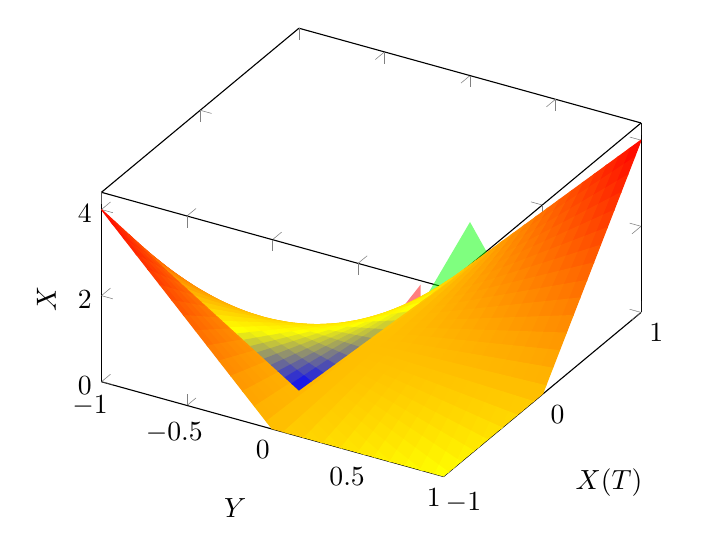
\begin{tikzpicture}
  \begin{axis}[view={60}{-45},
  %axis equal image=true,
  xlabel=$X(T)$, ylabel={$Y$}, zlabel={$X$},
  zmin=0
  ]
  \fill[opacity=0.5,red] (axis cs: 0,0,0) -- (axis cs: 0.5,0,0.5) -- (axis cs: 0.5,0,0) -- cycle;
  \fill[opacity=0.5,yellow] (axis cs: 0,0,0) -- (axis cs: 0,0.5,0.5) -- (axis cs: 0,0.5,0) -- cycle;
  \fill[opacity=0.5,green] (axis cs: 1,0,1) -- (axis cs: 0.5,0.5,1) -- (axis cs: 0.5,0.5,0) -- (axis cs: 0.5,0,0) -- cycle;
  \fill[opacity=0.5,blue] (axis cs: 0,0.5,0.5) -- (axis cs: 0.5,0.5,1) -- (axis cs: 0.5,0.5,0) -- (axis cs: 0,0.5,0) -- cycle;
  \addplot3[surf,shader=flat,z buffer=sort,samples=30,domain=-1:1,y domain=-1:1]{4*x*y};
  \end{axis}
\end{tikzpicture}
\end{center}

\printbibliography{}
\end{document}
